\documentclass[border=10pt]{standalone}
\usepackage[svgnames]{xcolor}
\usepackage{amsmath}
\usepackage{pgfplots}
\pgfplotsset{compat=newest}
\usepackage[sfdefault]{FiraSans}
\usepackage{FiraMono}
\renewcommand*\familydefault{\sfdefault}
\begin{document}
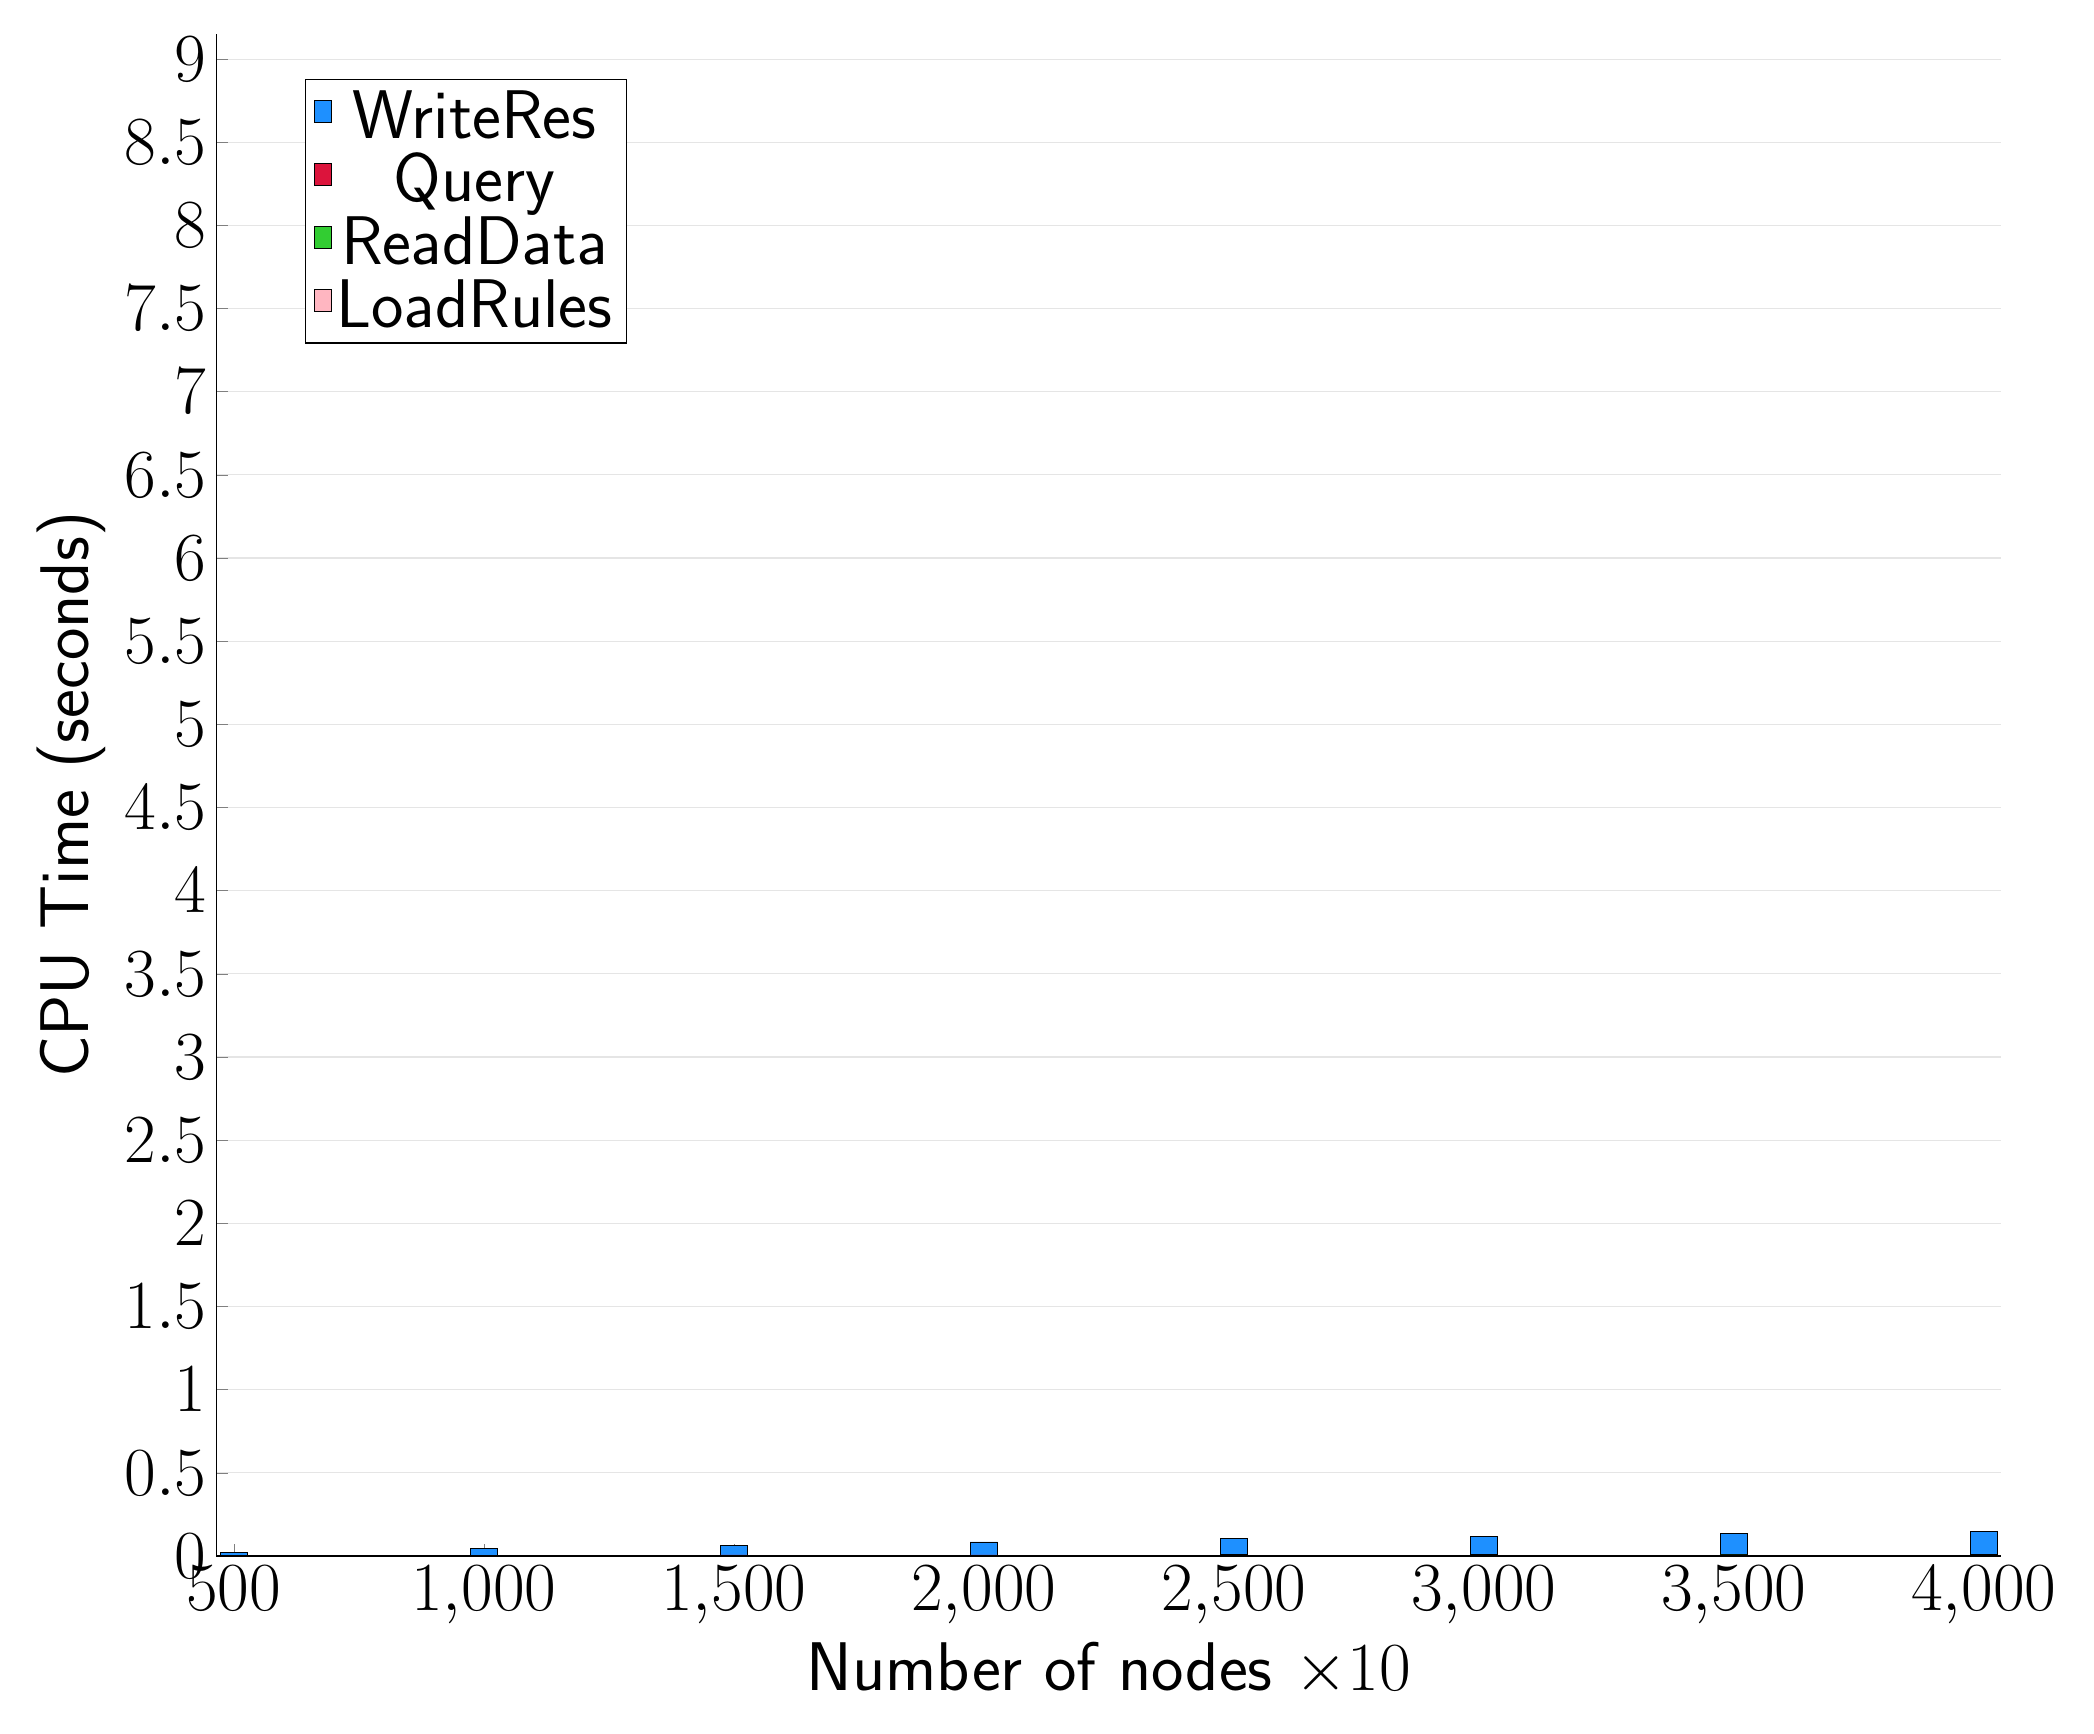
\begin{tikzpicture}
\begin{axis}[
   ybar stacked,
   width=2\textwidth,
   bar width=0.35cm,
   ymajorgrids, tick align=inside,
   major grid style={draw=gray!20},
   xtick=data,
   ymin=0, ymax=9.153333336114883,
   axis x line*=bottom,
   axis y line*=left,
   enlarge x limits=0.01,
   legend style={
       at={(0.23, 0.97)},
       anchor=north east,
       legend columns=1,
       font=\Huge,
   },
   ylabel={CPU Time (seconds)},
   xlabel={Number of nodes $\times 10$},
   label style={font=\Huge},
   tick label style={font=\Huge},
]
\addlegendimage{fill=DodgerBlue, draw=black, line width=0.2pt}
\addlegendentry{WriteRes}
\addlegendimage{fill=Crimson, draw=black, line width=0.2pt}
\addlegendentry{Query}
\addlegendimage{fill=LimeGreen, draw=black, line width=0.2pt}
\addlegendentry{ReadData}
\addlegendimage{fill=LightPink, draw=black, line width=0.2pt}
\addlegendentry{LoadRules}
\addplot +[fill=LightPink, draw=black, line width=0.2pt] coordinates {
(500, 0.0032156666666666666)
(1000, 0.0026676666666666667)
(1500, 0.0031873333333333333)
(2000, 0.0032736666666666665)
(2500, 0.0041080000000000005)
(3000, 0.003396)
(3500, 0.002521)
(4000, 0.003336)
};
\addplot +[fill=LimeGreen, draw=black, line width=0.2pt] coordinates {
(500, 0.001319666666666667)
(1000, 0.001983333333333333)
(1500, 0.002572666666666667)
(2000, 0.0027886666666666667)
(2500, 0.004228)
(3000, 0.004048)
(3500, 0.0040876666666666665)
(4000, 0.005007999999999999)
};
\addplot +[fill=Crimson, draw=black, line width=0.2pt] coordinates {
(500, 0.000133000000000001)
(1000, 0.000271999999999999)
(1500, 0.00041433333333333366)
(2000, 0.00034633333333333266)
(2500, 0.0007863333333333333)
(3000, 0.000765333333333332)
(3500, 0.0008849999999999986)
(4000, 0.0011076666666666667)
};
\addplot +[fill=DodgerBlue, draw=black, line width=0.2pt] coordinates {
(500, 0.018907)
(1000, 0.038862)
(1500, 0.05775566666666667)
(2000, 0.07807866666666667)
(2500, 0.09913633333333333)
(3000, 0.10946766666666667)
(3500, 0.12635366666666667)
(4000, 0.13916366666666666)
};
\end{axis}
\end{tikzpicture}

\end{document}
